\documentclass[11pt]{article}
\usepackage[textwidth=18.0cm, textheight=23.0cm, top=2.0cm]{geometry}
\usepackage{pst-all}
\usepackage{amssymb}
\usepackage{tikz}
\usepackage{underscore}\begin{document}
\pagestyle{empty}


ClassName: \underline{\textbf{Class_10.2bp-3}}
\par
BinSize: \underline{\textbf{100 × 100}}
\par
ReduceSize: \underline{\textbf{100 × 100}}
\par
TypeNum: \underline{\textbf{20}}
\par
Num: \underline{\textbf{20}}
\par
OutS: \underline{\textbf{50000}}
\par
InS: \underline{\textbf{33945}}
\par
Rate: \underline{\textbf{0.679}}
\par
UB: \underline{\textbf{5}}
\par
LB0: \underline{\textbf{5}}
\par
LB: \underline{\textbf{5}}
\par
LBWithCut: \underline{\textbf{5}}
\par
NodeCut: \underline{\textbf{0}}
\par
ExtendedNodeCnt: \underline{\textbf{1}}
\par
GenNodeCnt: \underline{\textbf{1}}
\par
PrimalNode: \underline{\textbf{0}}
\par
ColumnCount: \underline{\textbf{5}}
\par
TotalCutCount: \underline{\textbf{0}}
\par
RootCutCount: \underline{\textbf{0}}
\par
LPSolverCnt: \underline{\textbf{1}}
\par
PricingSolverCnt: \underline{\textbf{0}}
\par
BranchAndBoundNum: \underline{\textbf{1}}
\par
isOpt: \underline{\textbf{true}}
\par
TimeOnPrimal: \underline{\textbf{0.000 s}}
\par
TimeOnPricing: \underline{\textbf{0.000 s}}
\par
TimeOnRmp: \underline{\textbf{0.094 s}}
\par
TotalTime: \underline{\textbf{0.156 s}}
\par
\newpage


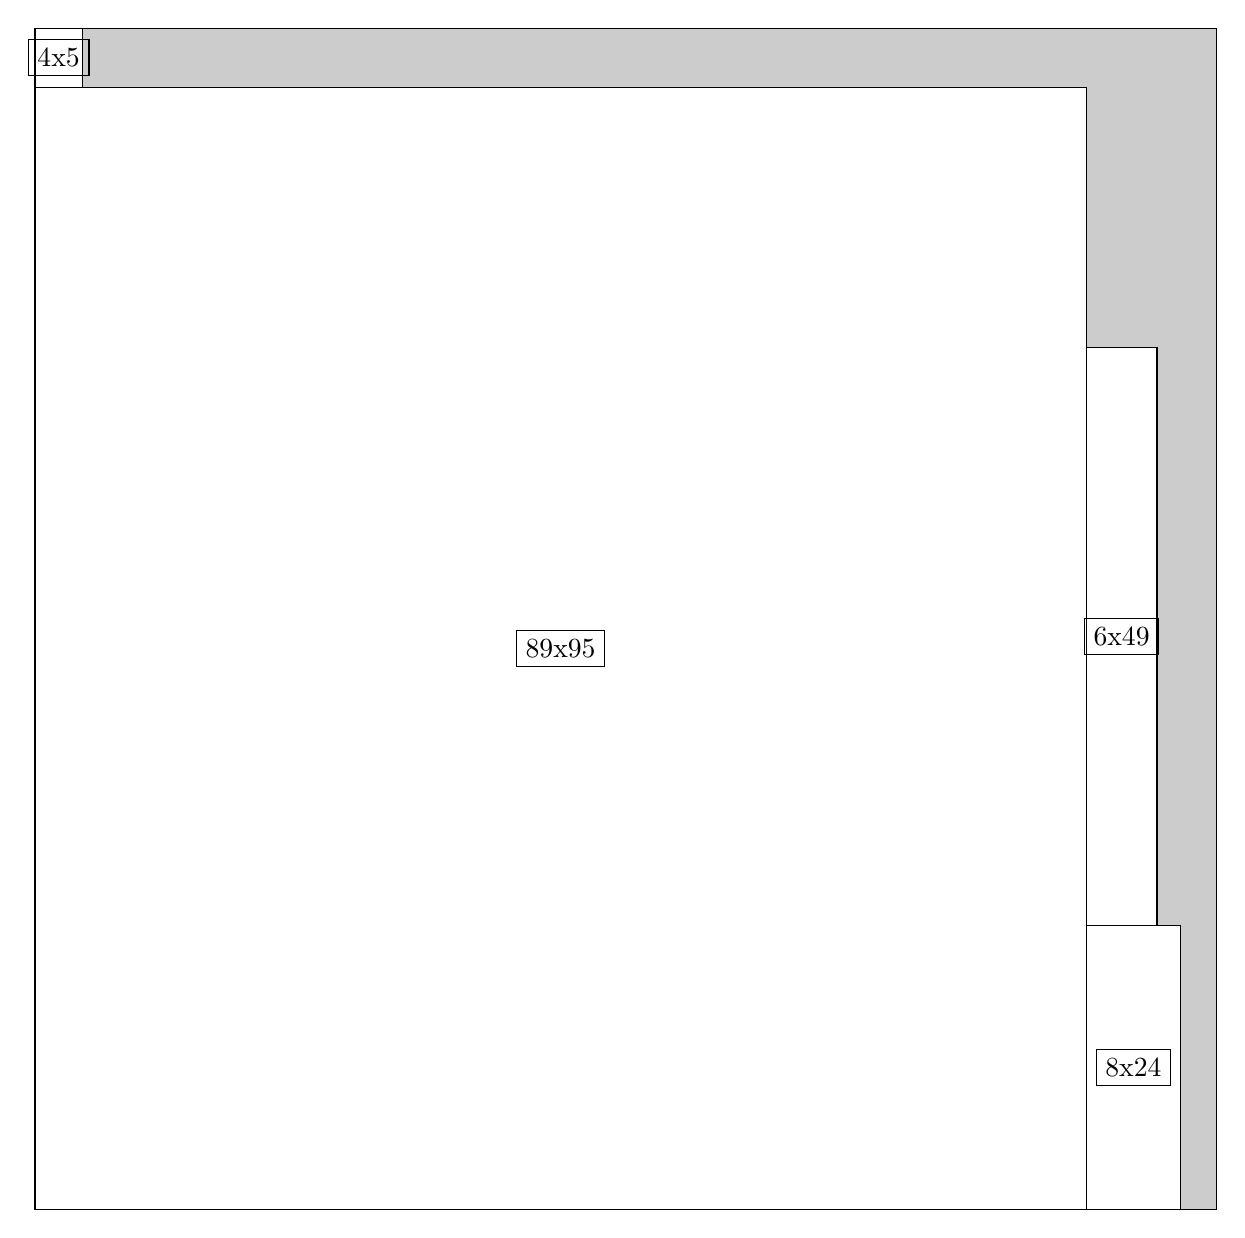
\begin{tikzpicture}[shorten >=1pt,scale=1.0,every node/.style={scale=1.0},->]
\tikzstyle{vertex}=[circle,fill=black!25,minimum size=14pt,inner sep=0pt]
\filldraw[fill=gray!40!white, draw=black] (0,0) rectangle (15.0,15.0);
\foreach \name/\x/\y/\w/\h in {89x95/0.0/0.0/13.35/14.25,6x49/13.35/3.5999999999999996/0.8999999999999999/7.35,8x24/13.35/0.0/1.2/3.5999999999999996,4x5/0.0/14.25/0.6/0.75}
\filldraw[fill=white!40!white, draw=black] (\x,\y) rectangle node[draw] (\name) {\name} ++(\w,\h);
\end{tikzpicture}


w =89 , h =95 , x =0 , y =0 , v =8455
\par
w =6 , h =49 , x =89 , y =24 , v =294
\par
w =8 , h =24 , x =89 , y =0 , v =192
\par
w =4 , h =5 , x =0 , y =95 , v =20
\par
\newpage


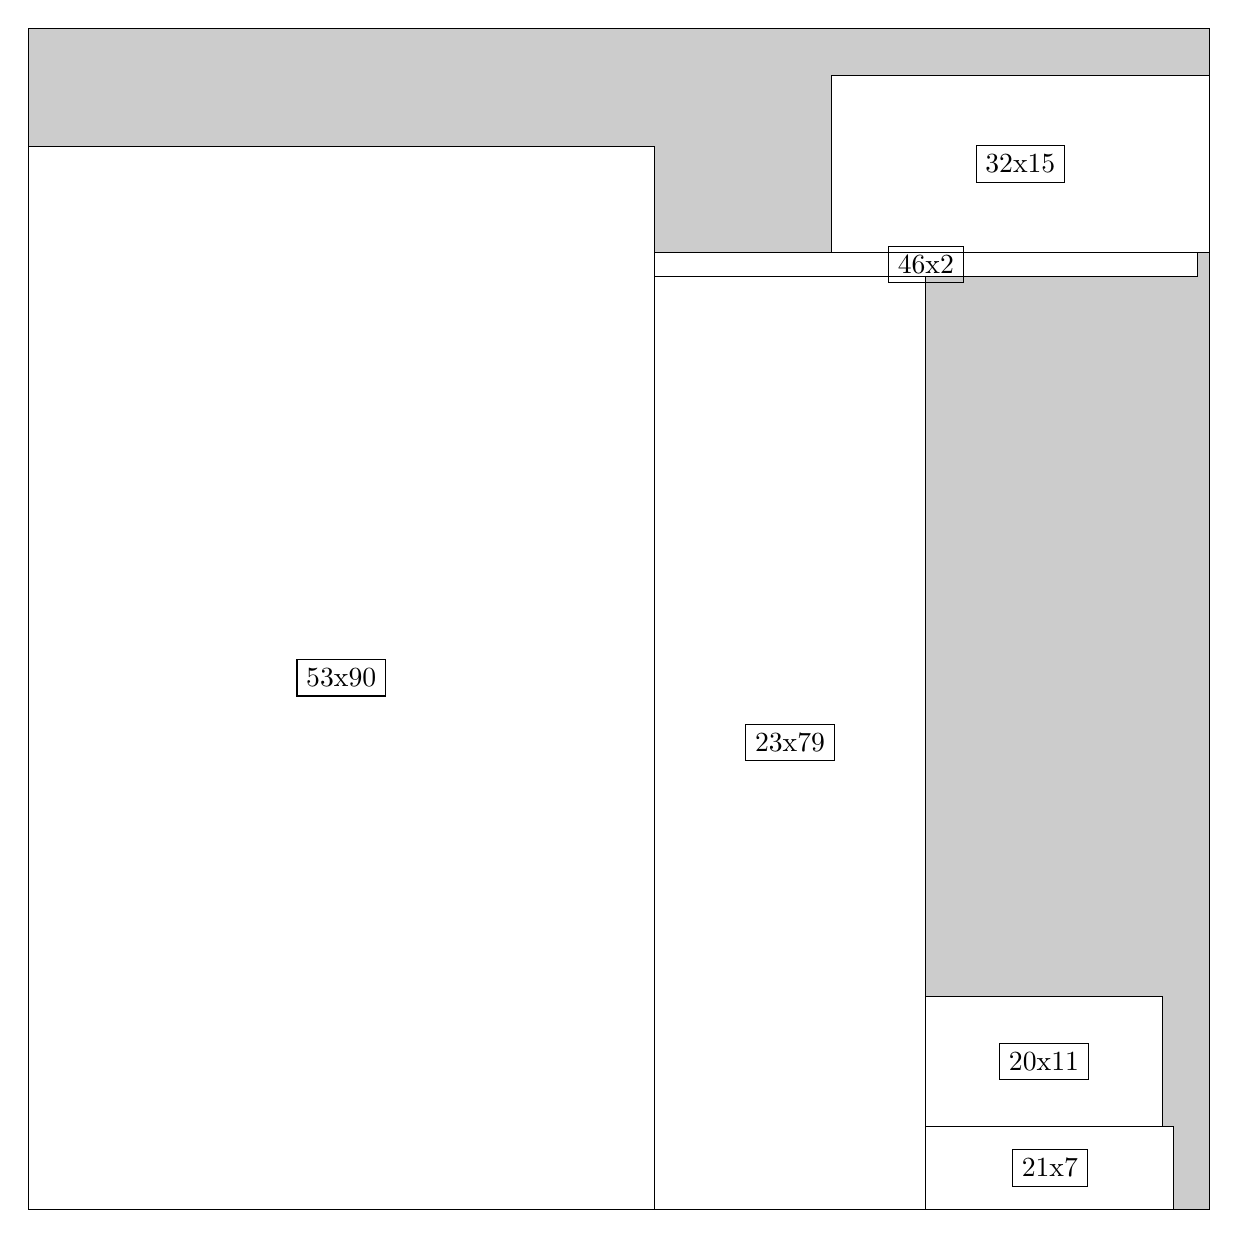
\begin{tikzpicture}[shorten >=1pt,scale=1.0,every node/.style={scale=1.0},->]
\tikzstyle{vertex}=[circle,fill=black!25,minimum size=14pt,inner sep=0pt]
\filldraw[fill=gray!40!white, draw=black] (0,0) rectangle (15.0,15.0);
\foreach \name/\x/\y/\w/\h in {53x90/0.0/0.0/7.949999999999999/13.5,23x79/7.949999999999999/0.0/3.4499999999999997/11.85,32x15/10.2/12.15/4.8/2.25,20x11/11.4/1.05/3.0/1.65,46x2/7.949999999999999/11.85/6.8999999999999995/0.3,21x7/11.4/0.0/3.15/1.05}
\filldraw[fill=white!40!white, draw=black] (\x,\y) rectangle node[draw] (\name) {\name} ++(\w,\h);
\end{tikzpicture}


w =53 , h =90 , x =0 , y =0 , v =4770
\par
w =23 , h =79 , x =53 , y =0 , v =1817
\par
w =32 , h =15 , x =68 , y =81 , v =480
\par
w =20 , h =11 , x =76 , y =7 , v =220
\par
w =46 , h =2 , x =53 , y =79 , v =92
\par
w =21 , h =7 , x =76 , y =0 , v =147
\par
\newpage


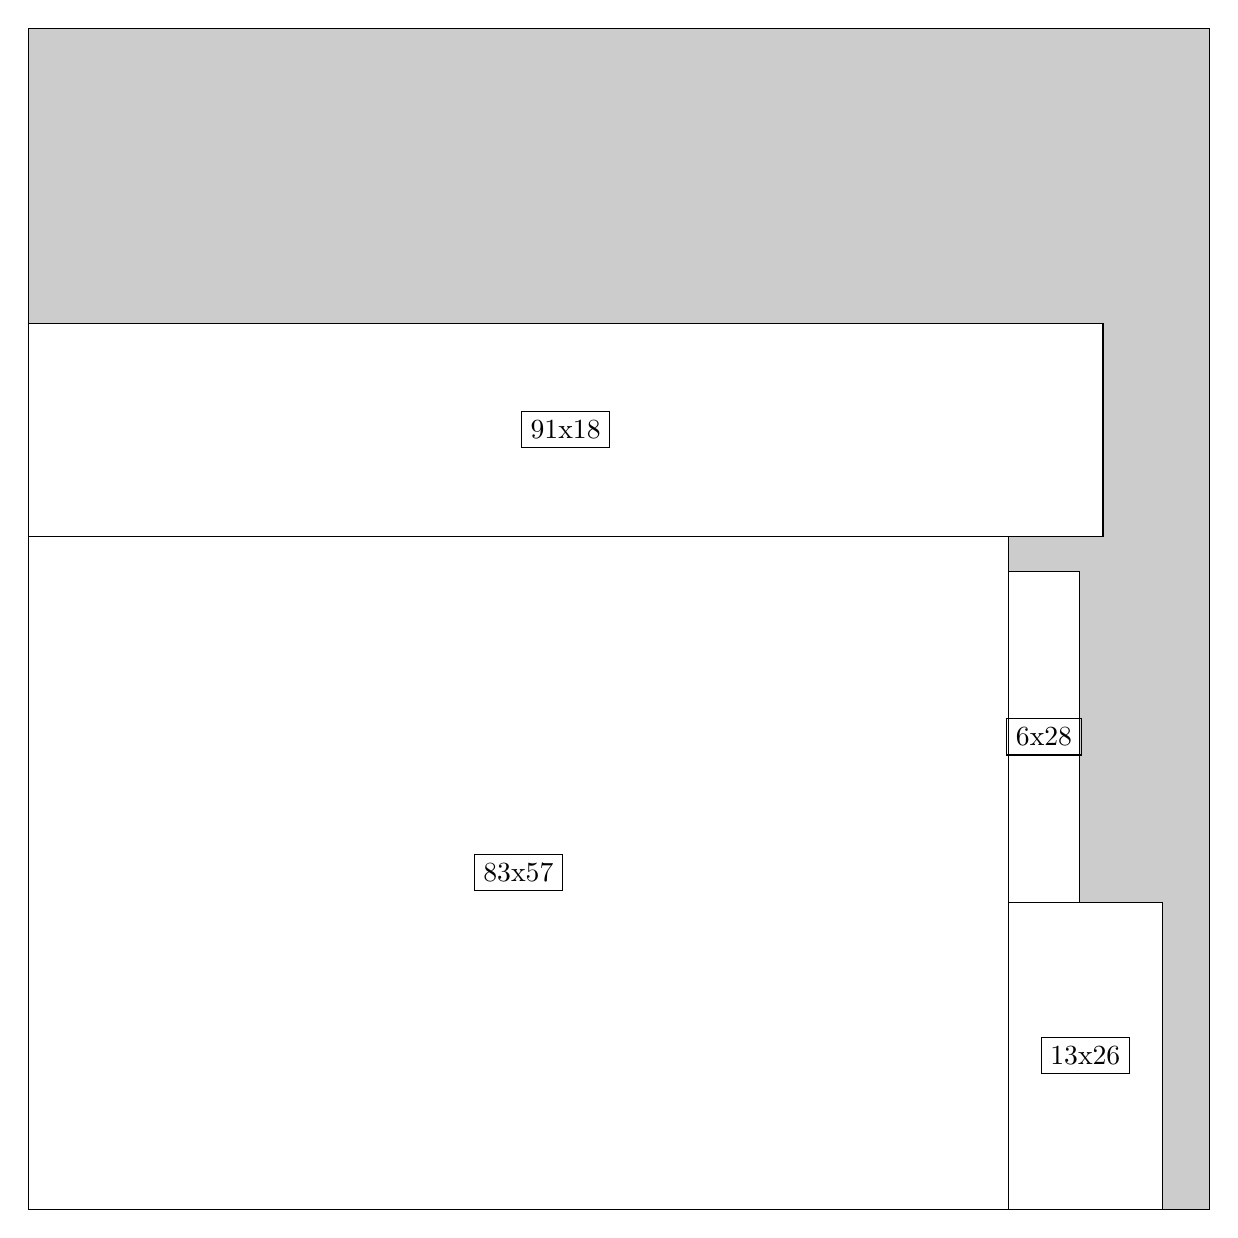
\begin{tikzpicture}[shorten >=1pt,scale=1.0,every node/.style={scale=1.0},->]
\tikzstyle{vertex}=[circle,fill=black!25,minimum size=14pt,inner sep=0pt]
\filldraw[fill=gray!40!white, draw=black] (0,0) rectangle (15.0,15.0);
\foreach \name/\x/\y/\w/\h in {83x57/0.0/0.0/12.45/8.549999999999999,91x18/0.0/8.549999999999999/13.65/2.6999999999999997,13x26/12.45/0.0/1.95/3.9,6x28/12.45/3.9/0.8999999999999999/4.2}
\filldraw[fill=white!40!white, draw=black] (\x,\y) rectangle node[draw] (\name) {\name} ++(\w,\h);
\end{tikzpicture}


w =83 , h =57 , x =0 , y =0 , v =4731
\par
w =91 , h =18 , x =0 , y =57 , v =1638
\par
w =13 , h =26 , x =83 , y =0 , v =338
\par
w =6 , h =28 , x =83 , y =26 , v =168
\par
\newpage


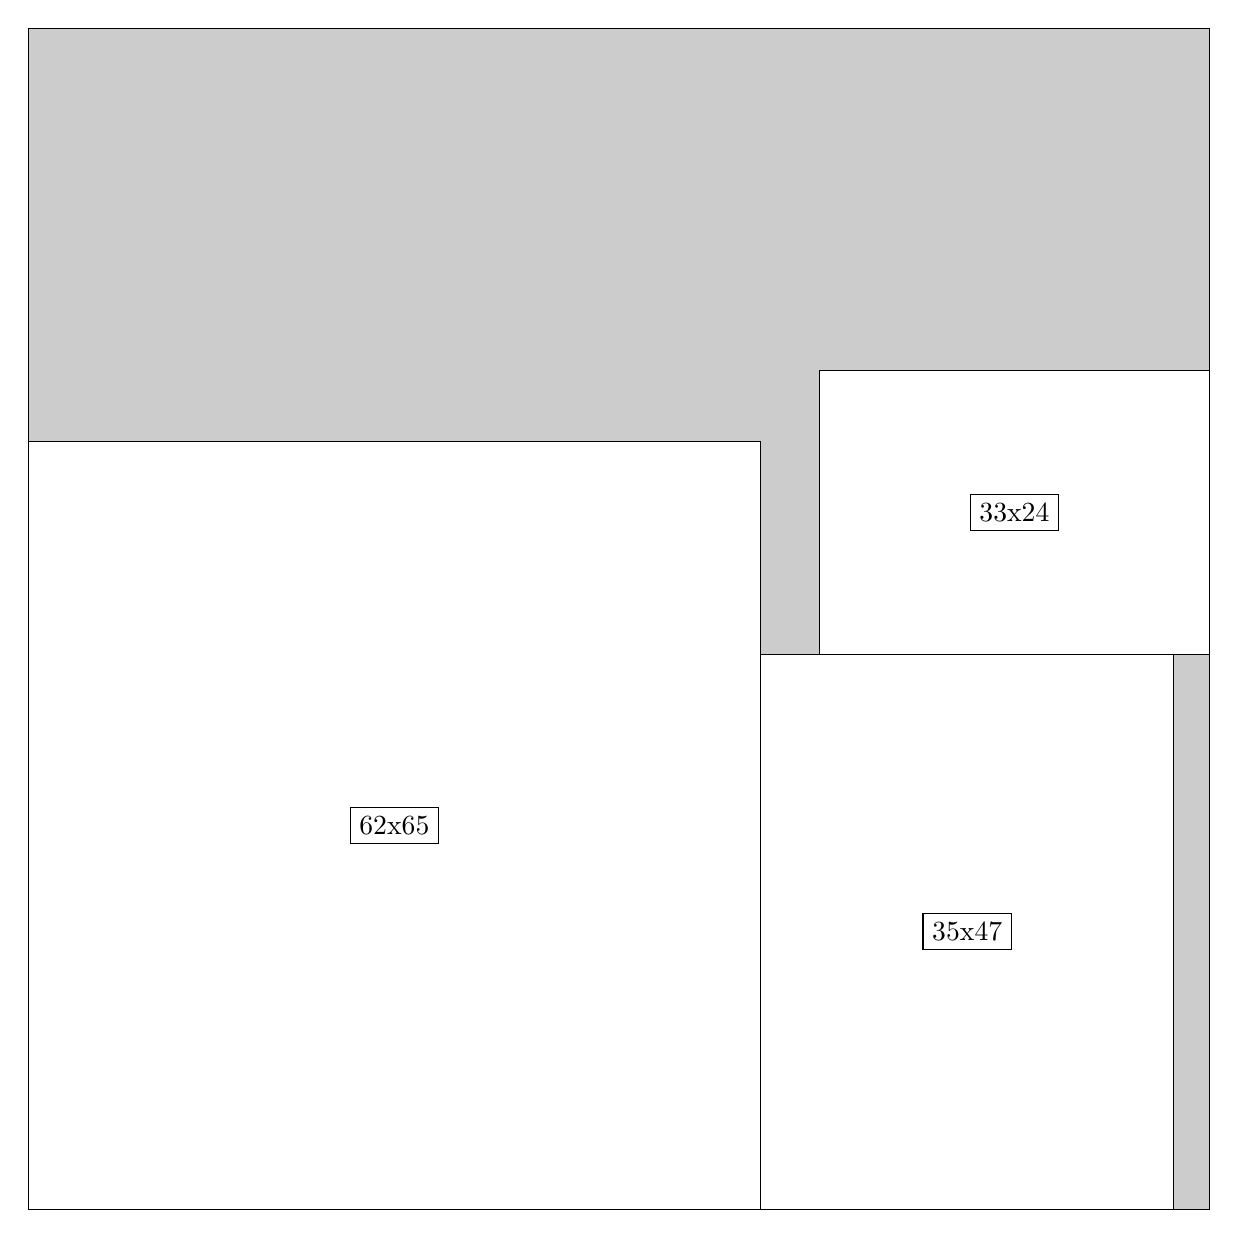
\begin{tikzpicture}[shorten >=1pt,scale=1.0,every node/.style={scale=1.0},->]
\tikzstyle{vertex}=[circle,fill=black!25,minimum size=14pt,inner sep=0pt]
\filldraw[fill=gray!40!white, draw=black] (0,0) rectangle (15.0,15.0);
\foreach \name/\x/\y/\w/\h in {62x65/0.0/0.0/9.299999999999999/9.75,35x47/9.299999999999999/0.0/5.25/7.05,33x24/10.049999999999999/7.05/4.95/3.5999999999999996}
\filldraw[fill=white!40!white, draw=black] (\x,\y) rectangle node[draw] (\name) {\name} ++(\w,\h);
\end{tikzpicture}


w =62 , h =65 , x =0 , y =0 , v =4030
\par
w =35 , h =47 , x =62 , y =0 , v =1645
\par
w =33 , h =24 , x =67 , y =47 , v =792
\par
\newpage


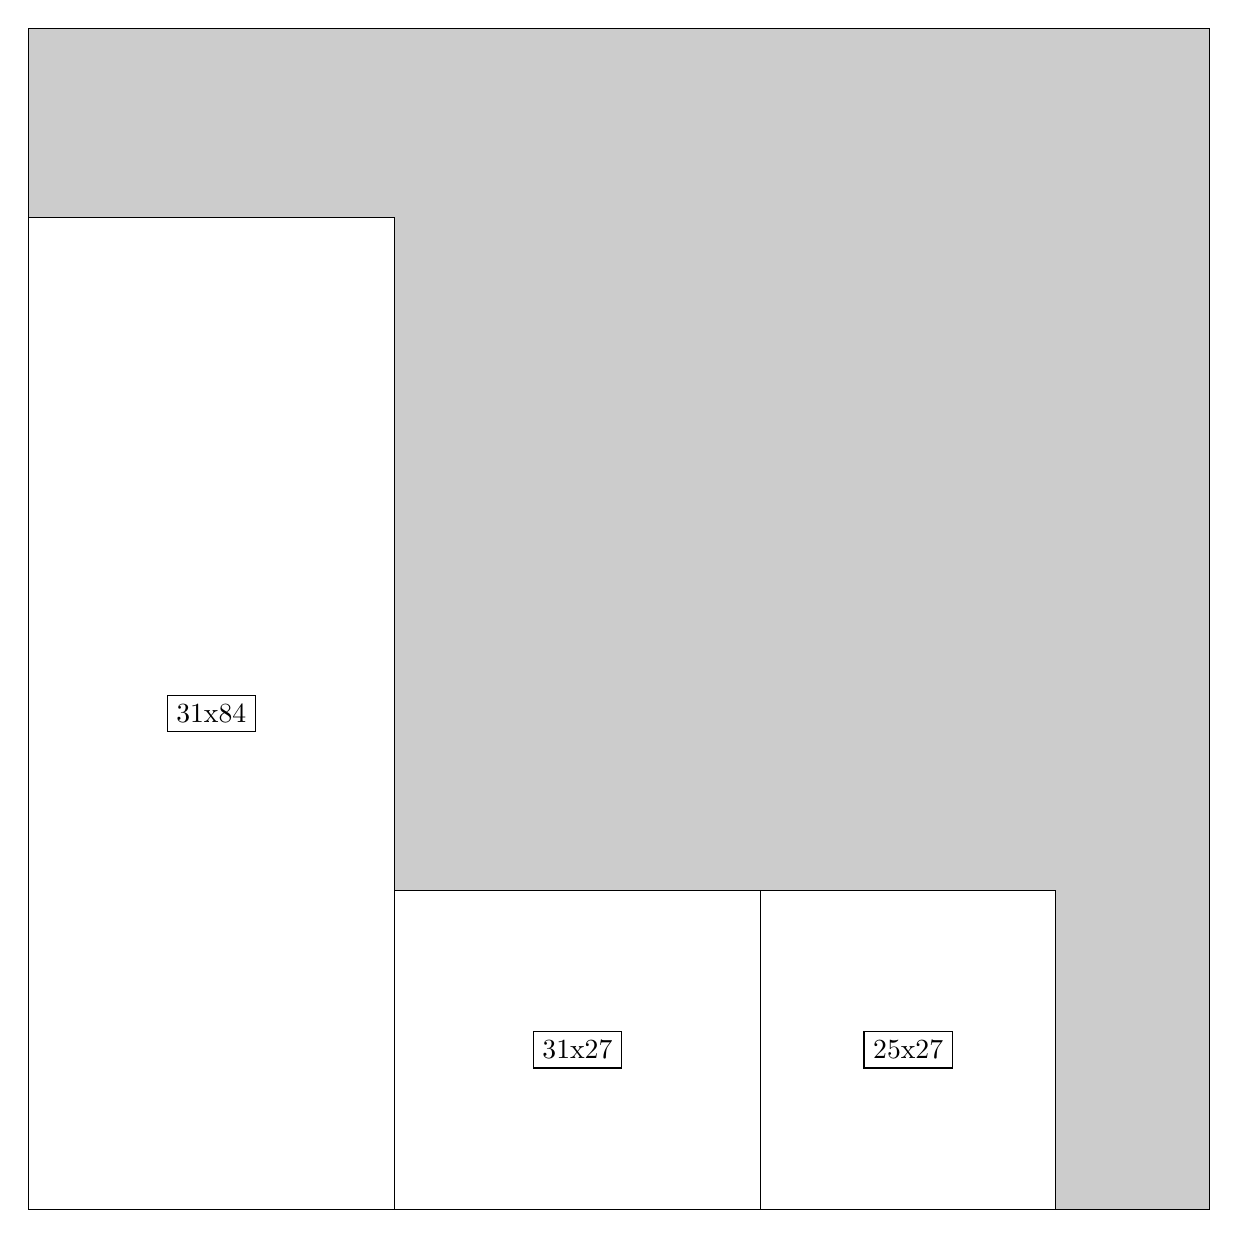
\begin{tikzpicture}[shorten >=1pt,scale=1.0,every node/.style={scale=1.0},->]
\tikzstyle{vertex}=[circle,fill=black!25,minimum size=14pt,inner sep=0pt]
\filldraw[fill=gray!40!white, draw=black] (0,0) rectangle (15.0,15.0);
\foreach \name/\x/\y/\w/\h in {31x84/0.0/0.0/4.6499999999999995/12.6,31x27/4.6499999999999995/0.0/4.6499999999999995/4.05,25x27/9.299999999999999/0.0/3.75/4.05}
\filldraw[fill=white!40!white, draw=black] (\x,\y) rectangle node[draw] (\name) {\name} ++(\w,\h);
\end{tikzpicture}


w =31 , h =84 , x =0 , y =0 , v =2604
\par
w =31 , h =27 , x =31 , y =0 , v =837
\par
w =25 , h =27 , x =62 , y =0 , v =675
\par
\newpage


\end{document}